\documentclass[aspectratio=169,10pt]{beamer}
\usepackage{../common/beamer_theme_bio}

\title{\textbf{Biostatistiques Appliquées}}
\subtitle{Chapitre 0 : Fondements, Variabilité Biologique \& Démarche Statistique}
\author{\textbf{Dr. Sarra BENMOUMOU (Ph.D.)}}
\institute{
  Faculté des Sciences --- Département de Biologie\\
  Master 2 : Biochimie Appliquée\\
  \textbf{Université M'Hamed Bougara de Boumerdès (UMBB)}
}
\date{Année Universitaire 2024 -- 2025}

\begin{document}

% --- Titre ---
\begin{frame}[plain]
  \titlepage
\end{frame}

% --- Sommaire ---
\begin{frame}{Plan Détaillé du Chapitre 0}
  \tableofcontents
\end{frame}

% ========================================================
\section{La Démarche Biostatistique en Biochimie}
% ========================================================

\begin{frame}{Pourquoi le Biochimiste a-t-il Besoin des Statistiques ?}
  \begin{columns}[onlytextwidth, T]
    \begin{column}{0.48\linewidth}
      \begin{conceptbox}{La Nature Intrinsèque du Vivant}
        En physique ou en chimie minérale, les réactions dans des conditions identiques donnent des résultats quasi-parfaits.\\
        \vspace{1mm}
        En \textbf{Biochimie et Biologie} :
        \begin{itemize}
          \item Deux souris consanguines réagissent différemment.
          \item Deux cultures cellulaires clonales présentent des micro-hétérogénéités d'expression enzymatique.
          \item Les cellules oscillent selon des rythmes métaboliques et circadiens.
        \end{itemize}
      \end{conceptbox}
    \end{column}
    \begin{column}{0.48\linewidth}
      \begin{biobox}{Le Rôle Central de la Statistique}
        La biostatistique n'est pas un ensemble de calculs abstraits ; c'est \textbf{l'outil décisionnel} permettant de :
        \begin{enumerate}
          \item \textbf{Quantifier l'incertitude} inhérente aux mesures expérimentales.
          \item \textbf{Séparer le signal biologique réel} du bruit de fond aléatoire.
          \item \textbf{Prendre une décision objective} : valider ou réfuter l'efficacité d'un traitement avec un risque d'erreur contrôlé.
        \end{enumerate}
      \end{biobox}
    \end{column}
  \end{columns}
\end{frame}

\begin{frame}{Décomposition de la Variabilité Expérimentale}
  \begin{conceptbox}{L'Équation Fondamentale du Laboratoire}
    Toute mesure brute $Y$ obtenue au spectrophotomètre, en cytométrie ou en ELISA s'écrit :
    \begin{equation*}
      \text{\textbf{Mesure Observée}} = \text{\textbf{Valeur Vraie}} + \text{\textbf{Biais Biologique}} + \text{\textbf{Erreur Technique}}
    \end{equation*}
  \end{conceptbox}

  \begin{columns}[onlytextwidth, T]
    \begin{column}{0.48\linewidth}
      \textbf{\color{BioTeal}\faDna\ Variabilité Biologique (Inhérente)}
      \begin{itemize}
        \item Diversité génétique et statut épigénétique.
        \item Âge, poids, cycle hormonal des animaux.
        \item $\implies$ \textbf{C'est l'objet même de l'étude scientifique !} On ne peut pas l'annuler, on doit l'estimer.
      \end{itemize}
    \end{column}
    \begin{column}{0.48\linewidth}
      \textbf{\color{BioAmber}\faVial\ Variabilité Technique (Artefactuelle)}
      \begin{itemize}
        \item Imprécision volumétrique des pipettes.
        \item Fluctuations thermiques de l'étuve.
        \item Dérive de la lampe UV-visible du lecteur.
        \item $\implies$ \textbf{Bruit parasite} à minimiser par de bonnes pratiques de laboratoire.
      \end{itemize}
    \end{column}
  \end{columns}
\end{frame}

\begin{frame}{Réplicats Biologiques vs. Réplicats Techniques}
  \begin{columns}[onlytextwidth, T]
    \begin{column}{0.48\linewidth}
      \begin{conceptbox}{Réplicats Biologiques ($N$)}
        Échantillons prélevés sur des \textbf{individus ou organismes totalement indépendants} (ex: 5 souris différentes, 3 extractions végétales distinctes).\\
        \vspace{1mm}
        $\implies$ \textbf{Seuls les réplicats biologiques} confèrent le droit de généraliser les conclusions à l'ensemble d'une espèce ou d'une population !
      \end{conceptbox}
    \end{column}
    \begin{column}{0.48\linewidth}
      \begin{warnbox}{Réplicats Techniques ($k$)}
        Mesures répétées sur le \textbf{même échantillon biologique} (ex : doser 3 fois le même extrait tissulaire dans 3 puits d'une plaque ELISA).\\
        \vspace{1mm}
        $\implies$ Réduit l'imprécision de pipetage, mais \textbf{ne donne aucune information} sur la variabilité inter-individuelle.
      \end{warnbox}
    \end{column}
  \end{columns}
  \vspace{1mm}
  \begin{takeawaybox}{La Pseudo-Réplication : Faute Déontologique Grave}
    Compter 3 mesures techniques sur 1 seule souris comme $n=3$ est une tromperie méthodologique. Le vrai $n$ biologique est 1 !
  \end{takeawaybox}
\end{frame}

% ========================================================
\section{Typologie des Variables en Biochimie}
% ========================================================

\begin{frame}{Les Différentes Natures de Données de Laboratoire}
  \begin{table}[h]
    \centering
    \small
    \resizebox{\linewidth}{!}{%
    \begin{tabular}{lp{6cm}p{5.5cm}}
      \toprule
      \textbf{Type de Variable} & \textbf{Définition \& Échelle} & \textbf{Exemples Précis en Biochimie} \\
      \midrule
      \textbf{Quantitative continue} & Valeurs réelles infinies sur un intervalle mesurable. & Absorbance ($A_{595}$), Concentration protéique ($\mu\text{g/mL}$), Activité enzymatique ($\mu\text{mol/min/mg}$), pH. \\
      \midrule
      \textbf{Quantitative discrète} & Nombres entiers résultant d'un comptage. & Nombre de colonies bactériennes (UFC), comptage cellulaire sur cellule de Malassez. \\
      \midrule
      \textbf{Qualitative nominale} & Catégories disjointes sans hiérarchie ni ordre. & Génotype (Sauvage WT vs Muté KO), Sexe, Type de tissu (Foie, Rein, Muscle). \\
      \midrule
      \textbf{Qualitative ordinale} & Classes possédant un ordre naturel ou gravité. & Stade de fibrose hépatique (F0, F1, F2, F3, F4), intensité de bande Western blot (+, ++, +++). \\
      \bottomrule
    \end{tabular}%
    }
  \end{table}
  \vspace{1mm}
  \begin{takeawaybox}{Impact sur le Choix des Tests}
    On n'applique jamais un test de Student ou une ANOVA sur des scores qualitatifs ordinaux sans transformation appropriée ou recours aux tests non paramétriques (Kruskal-Wallis, Mann-Whitney) !
  \end{takeawaybox}
\end{frame}

% ========================================================
\section{Paramètres Descriptifs : SD vs. SEM}
% ========================================================

\begin{frame}{Écart-Type (SD) vs. Erreur Standard (SEM) : Quelle Différence ?}
  \begin{columns}[onlytextwidth, T]
    \begin{column}{0.48\linewidth}
      \begin{conceptbox}{1. L'Écart-Type ($SD$)}
        \begin{equation*}
          SD = \sqrt{\frac{\sum_{i=1}^n (X_i - \bar{X})^2}{n - 1}}
        \end{equation*}
        \textbf{Signification biologique :} Mesure à quel point les individus biologiques sont dispersés autour de la moyenne.
        \begin{itemize}
          \item Ne diminue \textbf{pas} quand la taille d'échantillon $n$ augmente.
          \item Reflète la vraie diversité de la nature.
        \end{itemize}
      \end{conceptbox}
    \end{column}
    \begin{column}{0.48\linewidth}
      \begin{conceptbox}{2. L'Erreur Standard ($SEM$)}
        \begin{equation*}
          SEM = \frac{SD}{\sqrt{n}}
        \end{equation*}
        \textbf{Signification biologique :} Mesure l'incertitude sur la position de la moyenne vraie de la population ($\mu$).
        \begin{itemize}
          \item Diminue quand $n$ augmente ($\sim 1/\sqrt{n}$).
          \item Reflète la précision expérimentale.
        \end{itemize}
      \end{conceptbox}
    \end{column}
  \end{columns}
\end{frame}

\begin{frame}{Illustration Graphique : SD vs. SEM}
  \begin{center}
    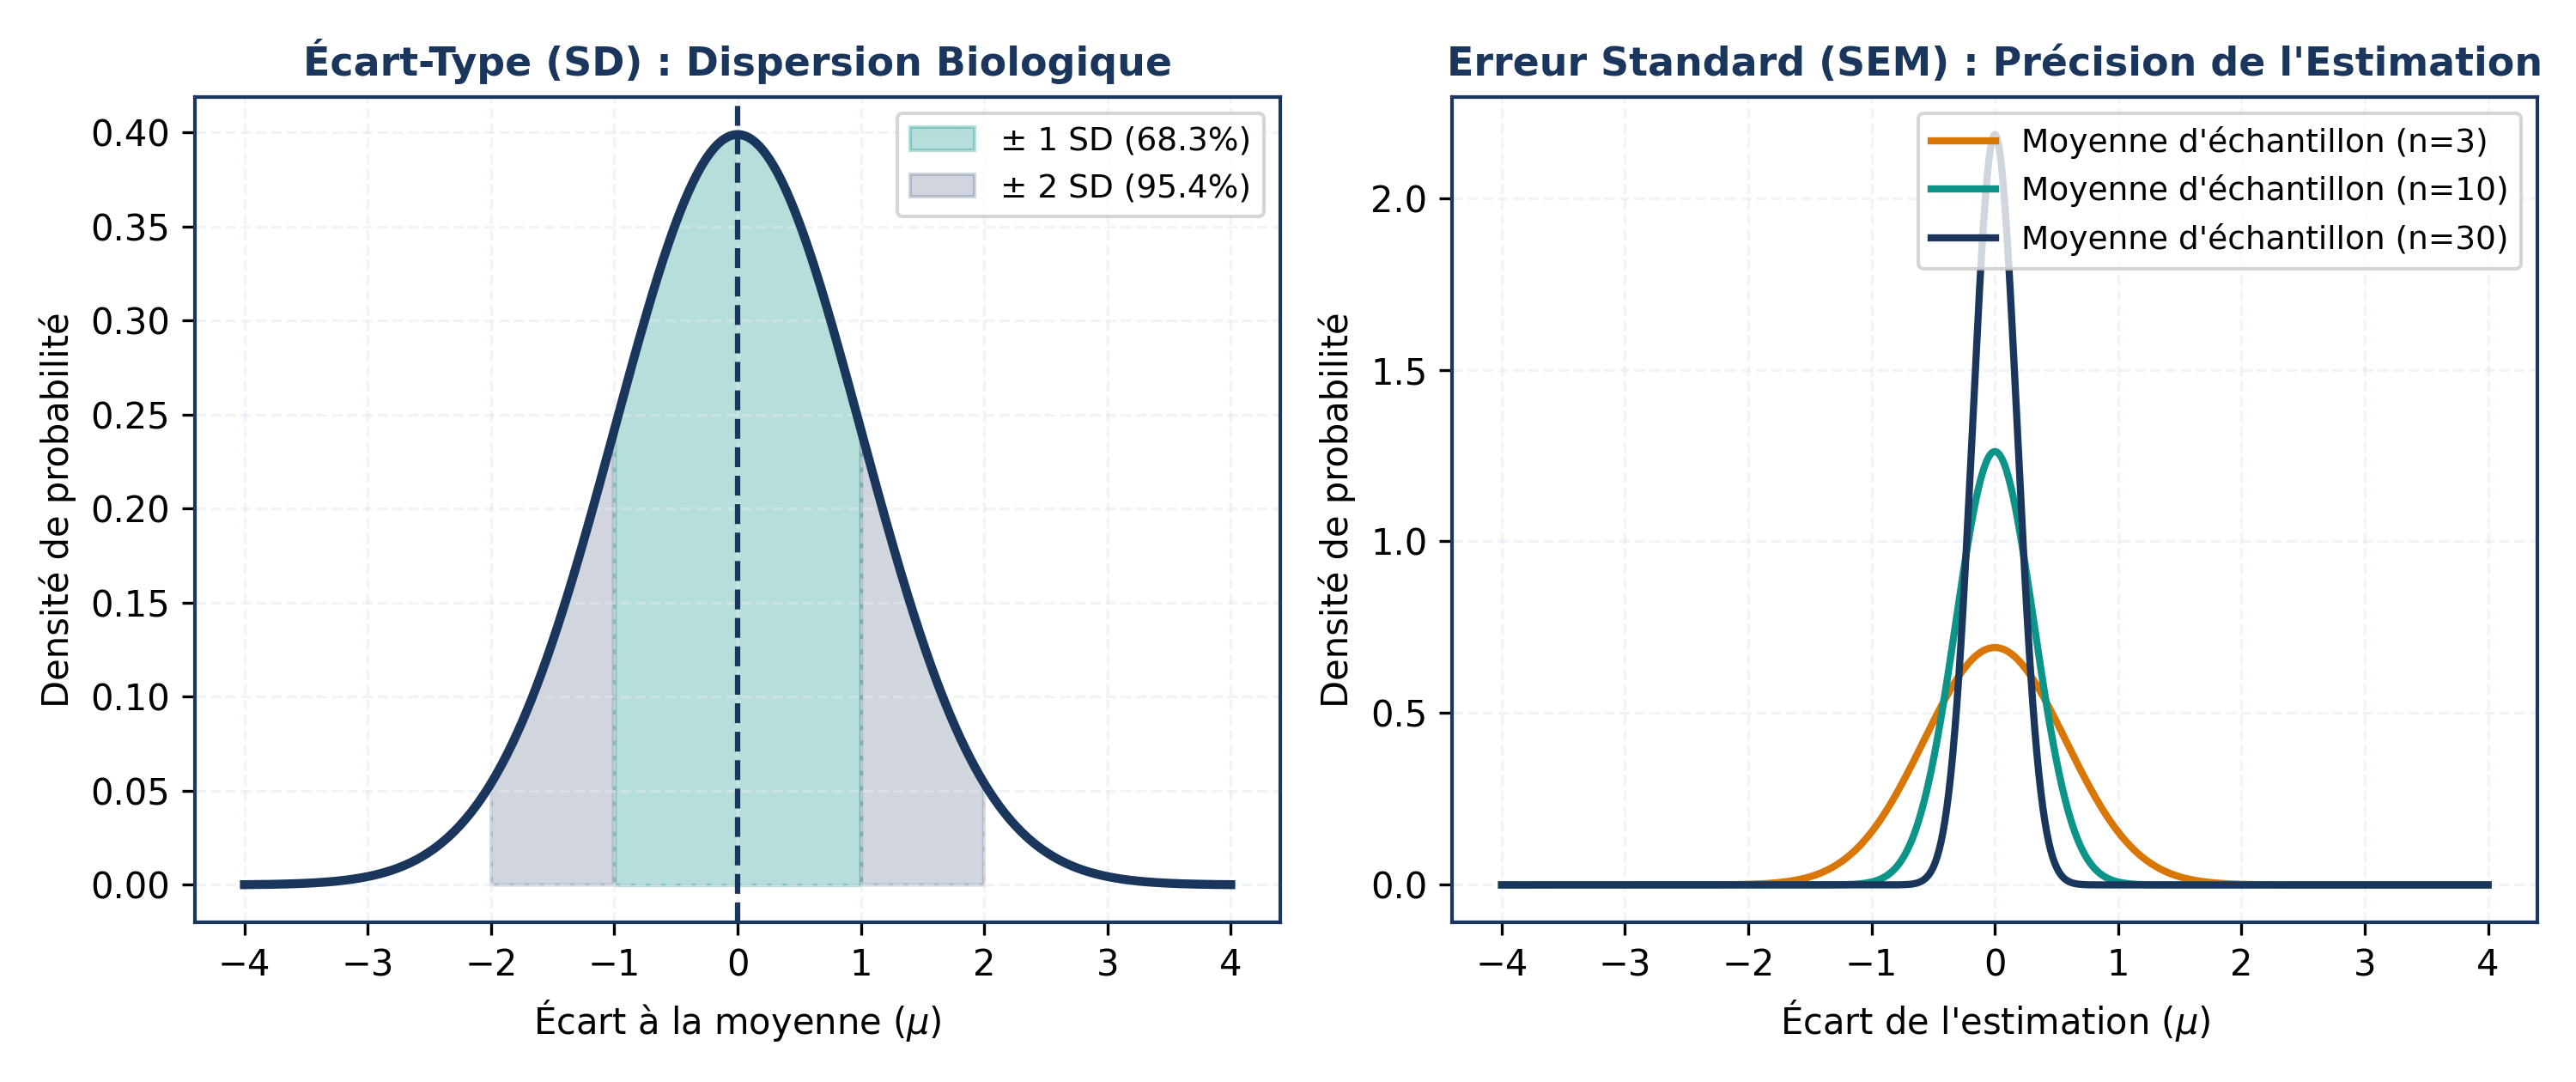
\includegraphics[width=0.90\linewidth]{../figures/fig00_distributions_sd_sem.png}
  \end{center}
  \vspace{-2mm}
  \begin{takeawaybox}{Recommandation Internationale}
    Si vous décrivez les caractéristiques d'un groupe d'animaux : indiquez $\text{Moyenne} \pm SD$. Si vous comparez l'effet de deux traitements : indiquez $\text{Moyenne} \pm SEM$ ou mieux, affichez l'intervalle de confiance à 95\% !
  \end{takeawaybox}
\end{frame}

% ========================================================
\section{La Logique des Tests d'Hypothèses}
% ========================================================

\begin{frame}{Le Raisonnement par l'Absurde du Test Statistique}
  \begin{columns}[onlytextwidth, T]
    \begin{column}{0.48\linewidth}
      \begin{conceptbox}{1. Formulation des Hypothèses}
        On ne peut jamais prouver directement qu'un traitement fonctionne. On cherche à \textbf{rejeter l'hypothèse qu'il ne fonctionne pas} :
        \begin{itemize}
          \item \textbf{$H_0$ (Hypothèse Nulle) :} « Pas de différence » ($\mu_A = \mu_B$).
          \item \textbf{$H_1$ (Alternative) :} « Il existe un effet » ($\mu_A \neq \mu_B$).
        \end{itemize}
      \end{conceptbox}
    \end{column}
    \begin{column}{0.48\linewidth}
      \begin{biobox}{Exemple en Enzymologie}
        On teste si un inhibiteur à $10\,\mu\text{M}$ réduit l'activité d'une protéase :
        \begin{equation*}
          H_0 : \text{Activité}_{\text{Inhibiteur}} = \text{Activité}_{\text{Témoin}}
        \end{equation*}
        Si la différence observée est tellement grande qu'elle a moins de 5\% de chances d'être due au hasard, on rejette $H_0$ !
      \end{biobox}
    \end{column}
  \end{columns}
\end{frame}

\begin{frame}{Les Deux Risques d'Erreur : $\alpha$, $\beta$ et Puissance}
  \begin{center}
    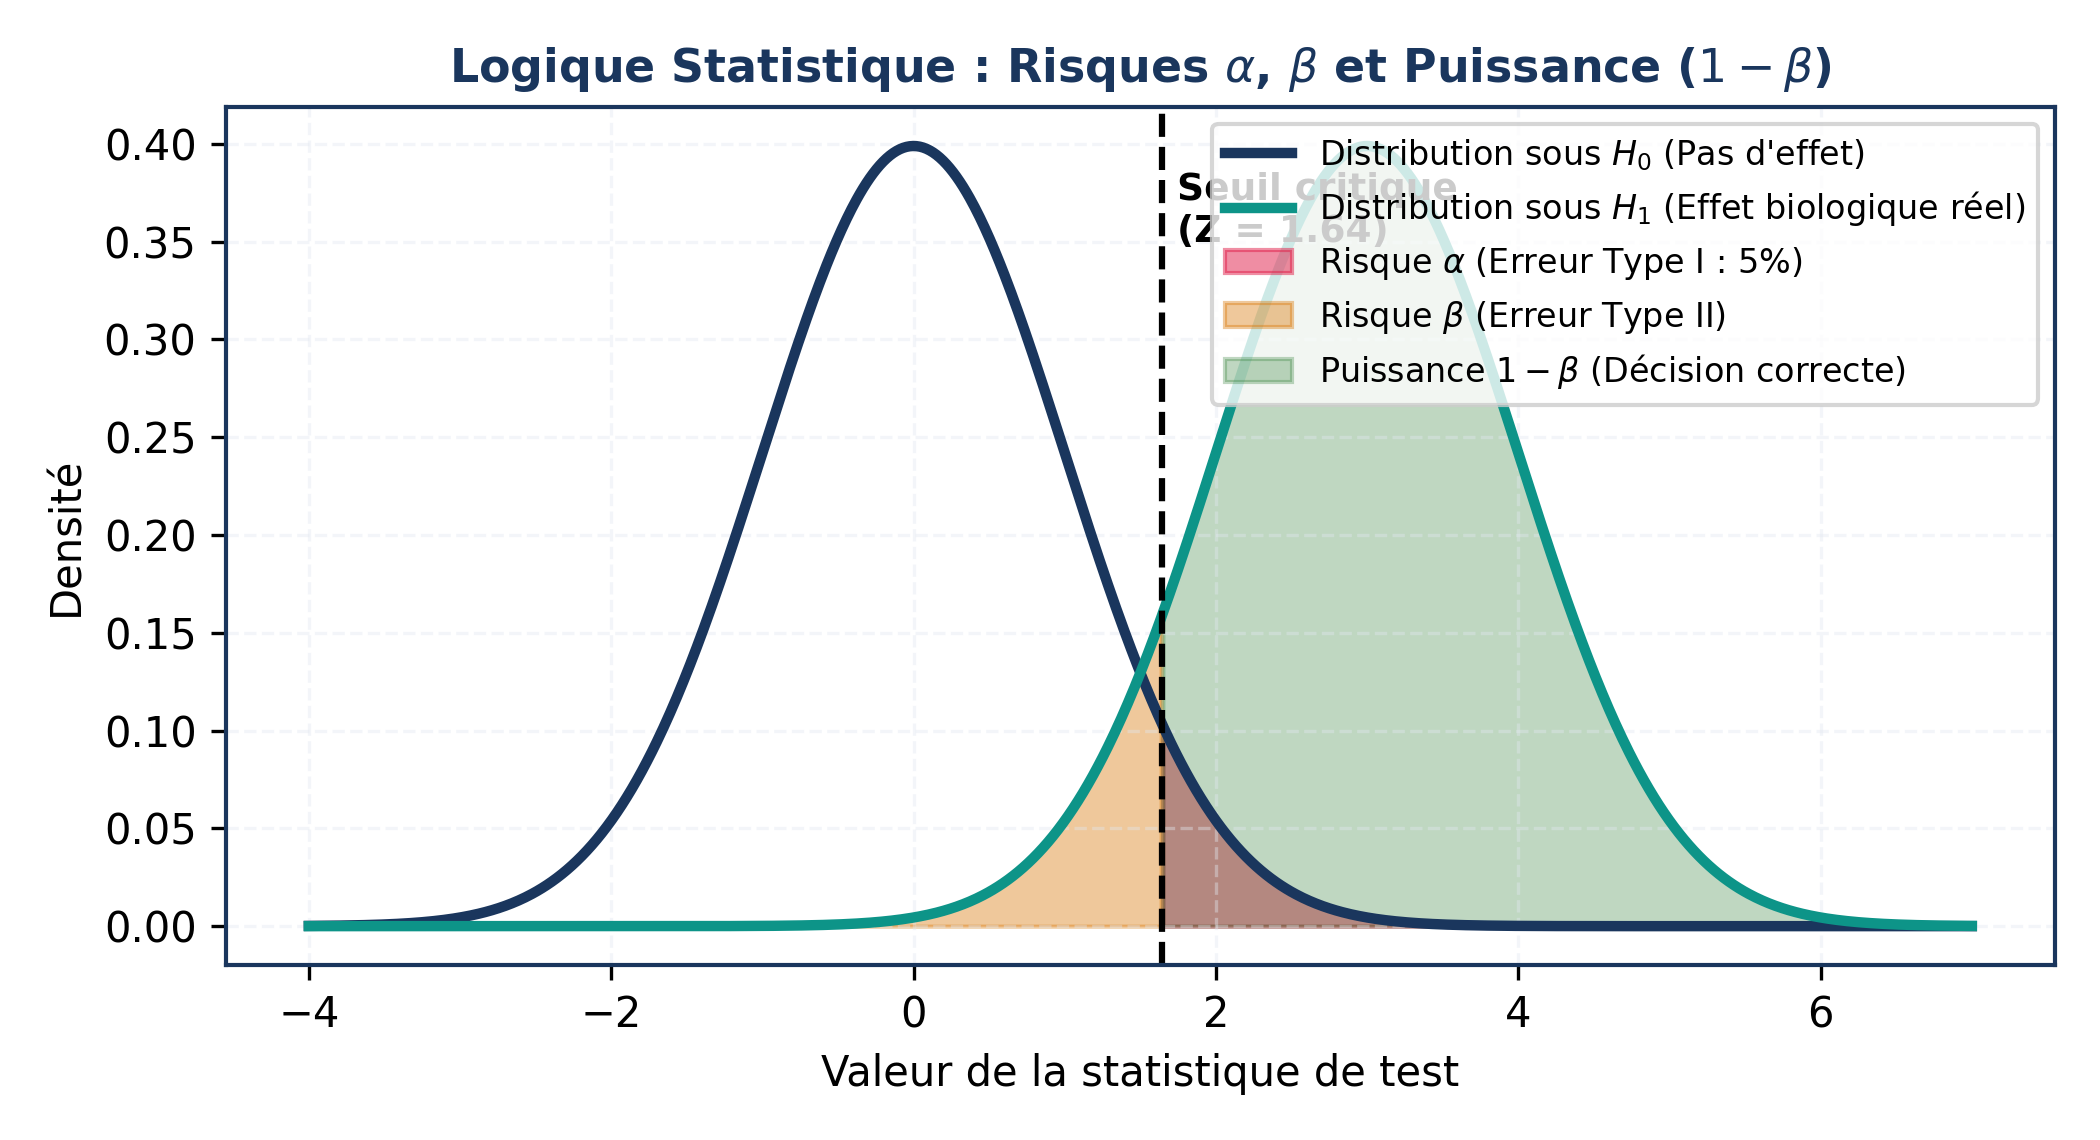
\includegraphics[width=0.78\linewidth]{../figures/fig00_hypothesis_testing_alpha_beta.png}
  \end{center}
  \vspace{-2mm}
  \begin{table}[h]
    \centering
    \scriptsize
    \resizebox{0.92\linewidth}{!}{%
    \begin{tabular}{p{3.5cm}|p{4.5cm}p{4.5cm}}
      \toprule
      \textbf{Décision du Chercheur} & \textbf{Réalité : $H_0$ est Vraie (Pas d'effet)} & \textbf{Réalité : $H_0$ est Fausse (Effet réel)} \\
      \midrule
      \textbf{Rejet de $H_0$ (Effet affirmé)} & \cellcolor{BioRed!25}\textbf{Erreur de Type I ($\alpha$, Faux Positif)} & \cellcolor{BioGreen!25}\textbf{Décision Correcte (Puissance $1-\beta$)} \\
      \textbf{Non-rejet de $H_0$ (Pas d'effet)} & \cellcolor{BioGreen!25}\textbf{Décision Correcte ($1-\alpha$)} & \cellcolor{BioAmber!25}\textbf{Erreur de Type II ($\beta$, Faux Négatif)} \\
      \bottomrule
    \end{tabular}%
    }
  \end{table}
\end{frame}

\begin{frame}{Démystification Rigoureuse de la $p$-value}
  \begin{conceptbox}{Définition Exacte}
    La \textbf{$p$-value} est la probabilité d'observer une différence au moins aussi grande que celle mesurée au laboratoire, \textbf{sous l'hypothèse où le traitement n'a absolument aucun effet réel ($H_0$ vraie)}.
    \begin{equation*}
      p \le 0.05 \implies \text{Événement très rare sous } H_0 \implies \text{Rejet de } H_0 \text{ (Différence significative)}.
    \end{equation*}
  \end{conceptbox}

  \begin{columns}[onlytextwidth, T]
    \begin{column}{0.48\linewidth}
      \begin{warnbox}{Les 3 Idées Fausses Répandues}
        \begin{enumerate}
          \item « $p = 0.03$ signifie qu'il y a 97\% de chances que $H_1$ soit vraie » $\implies$ \textbf{FAUX !}
          \item « Une $p$-value très faible ($p < 0.0001$) prouve un effet biologique géant » $\implies$ \textbf{FAUX !} (Avec $n=10000$, un effet infinitésimal donne $p < 0.0001$).
        \end{enumerate}
      \end{warnbox}
    \end{column}
    \begin{column}{0.48\linewidth}
      \begin{takeawaybox}{Significativité vs Pertinence Clinique}
        Toujours dissocier :
        \begin{itemize}
          \item \textbf{Significativité statistique} (la $p$-value).
          \item \textbf{Pertinence biologique} : la taille de l'effet mesuré (ex : baisse de 45\% de la glycémie vs baisse de 0.5\%).
        \end{itemize}
      \end{takeawaybox}
    \end{column}
  \end{columns}
\end{frame}

% ========================================================
\section{Organisation \& Objectifs du Programme}
% ========================================================

\begin{frame}{Feuille de Route du Module de Biostatistiques}
  \begin{columns}[onlytextwidth, T]
    \begin{column}{0.48\linewidth}
      \textbf{\color{BioNavy}Partie I : Modèles Linéaires Avancés}
      \begin{itemize}
        \item \textbf{Chapitre I :} ANOVA croisée (détection d'interactions, synergie et antagonisme).
        \item \textbf{Chapitre II :} ANOVA hiérarchisée (variabilité technique vs biologique, contrôle qualité).
        \item \textbf{Chapitre III :} Régression linéaire \& étalonnages (LOD, LOQ, BSA/Bradford).
      \end{itemize}
      \vspace{2mm}
      \textbf{\color{BioNavy}Partie II : Modélisation Non Linéaire}
      \begin{itemize}
        \item \textbf{Chapitre IV :} Cinétiques enzymatiques (Michaelis-Menten direct, Hill, 4PL ELISA).
      \end{itemize}
    \end{column}
    \begin{column}{0.48\linewidth}
      \textbf{\color{BioTeal}Partie III : Analyse de Données Multivariées}
      \begin{itemize}
        \item \textbf{Chapitre V :} ACP (Analyse en Composantes Principales de données omiques).
        \item \textbf{Chapitre VI :} CAH (Classification Hiérarchique \& Heatmaps).
      \end{itemize}
      \vspace{2mm}
      \textbf{\color{BioGreen}Partie IV : Intégrité \& Travaux Pratiques}
      \begin{itemize}
        \item \textbf{Chapitre VII :} Design expérimental \& publication.
        \item \textbf{TP Python / Jupyter :} Pratique sur jeux de données réels de biochimie.
      \end{itemize}
    \end{column}
  \end{columns}
\end{frame}

\begin{frame}[plain]
  \begin{center}
    \vspace{1.8cm}
    {\Huge\color{BioNavy}\textbf{Fin du Chapitre 0}}\\[0.8cm]
    {\large Vous possédez les bases conceptuelles indispensables pour aborder l'ANOVA croisée.}\\[1.2cm]
    \textbf{Dr. Sarra BENMOUMOU (Ph.D.)}\\
    \small Faculté des Sciences --- Département de Biologie\\
    \textbf{Université M'Hamed Bougara de Boumerdès (UMBB)}
  \end{center}
\end{frame}

\end{document}
